\chapter{Graph-Datenbanken im praktischen Einsatz: \ac{OLTP}}
\section{PostgresSQL: OLTP}
Die Implementierung von OLTP Anwendungsfällen ist eine klassische Aufgabe für relationale Datenbanken.
Da statt einer Graphdatenbank eine relationale Datenbank verwendet wurde, ist die Implementierung des OLTP Anwendungsfalls (Gästebuch) uninteressant.
Interessant ist jedoch die Traversierung in relationalen Datenbanken.
Für die Graphtraversierung wurden eigene Scripte geschrieben, die in diesem Kapitel vorgestellt werden.
\subsection{Traversierung in PostgresSQL}
%Das Ziel ist es 5 Graphen mit Hilfe einer objektrelationalen Datenbank zu traversieren.
Da Graphdatenbanken für das Traversieren von Graphen entwickelt worden sind, sollten diese bei der Traversierung einen Performancegewinn gegenüber objektrelationalen Datenbanken haben.
%Die Vermutung ist, dass das Traversieren eines Graphen mit Hilfe einer objektrelationalen Datenbank ähnlich performant ist, wie das Traversieren mit Hilfe einer Graphdatenbank.
Ziel ist es mit Hilfe einer objektrelationalen Datenbank eine mit den Graphdatenbanken vergleichbar performante Abfrage eines Graphen zu implementieren.
Für die Graphtraversierung sind 5 Methoden vorgesehen:
\begin{itemize}
    \item Graphtraversierung mit Hilfe von Standard \ac{SQL} (SELECT RECURSIVE WITH UNION)
    \item Graphtraversierung mit Hilfe von verschachteltem SELECT Statement
    \item Graphtraversierung mit Hilfe von rekursiven INNER JOIN
    \item Graphtraversierung mit Hilfe von selbstgeschriebenen Stored Procedure
    \item Graphtraversierung mit Hilfe von dynamisch generiertem \ac{SQL}
\end{itemize}
\subsection{Installation}
PostgreSQL kann unter Ubuntu über die Paketverwaltung \ac{APT} installiert werden. Weiterhin wird eine Installation über die \ac{RPM}-Paketverwaltung angeboten. Im Rahmen dieser
Arbeit wird PostgreSQL Version 11 verwendet. Ein Parallelbetrieb verschiedener PostgreSQL Versionen ist möglich. Nach der Installation von PostgreSQL muss zunächst
$initdb$ ausgeführt werden. Über $initdb$ wird ein PostgreSQL-Cluster angelegt. Als Parameter kann ein Directory-Pfad angegeben werden.
In diesem Pfad wird der PostgreSQL-Cluster von $initdb$ angelegt. Gemäß der Vorgaben dieser Arbeit wurde das PostgreSQL-Cluster unter
$/data/team22/postgresql/11/main$ installiert.
\subsection{CSV-Import}
Beim Import von (CSV)-Dateien wird zwischen Import vom Clientsystem und  Import vom Serversystem unterschieden.
Für den Import vom Client wird das psql-Statement \textbackslash copy verwendet (siehe SQL Script \ref{copy}). \textbackslash copy liest Informationen aus einer Datei,
%@ToDo Hier Quelle genauer spezifizieren
die vom psql-Client aus erreichbar sein muss. \cite{postgres2018}

\subsection{Datenbankschema}
Für die Performancemessung sind 5 Graphen vorgesehen. Ein Graph besteht aus einer profiles Tabelle und einer relation Tabelle. Die beiden Tabelle werden mit Hilfe der
Spalte ID aus der jeweiligen profiles Tabelle verknüpft. Die Spalten src und dst aus der relation Tabelle sind Fremdschlüssel, sie verweisen auf die Spalte ID in der
profiles Tabelle. ID hingegen ist in der profiles Tabelle ein Primärschlüssel (siehe \ref{relationFacebook}).

\subsection{Erstellen von Fremdschlüsseln}
Um die profile Tabelle und die relation Tabelle zu verknüpfen wurde zwischen den beiden Tabellen ein Fremdschlüssel erstellt. Bei der Erstellung wurde die profile Tabelle
mit einem Zähler versehen. Hierbei wurde der postgres Befehl serial verwendet, der einen Zähler für jede Zeile der Tabelle erstellt und bei 1 startet . Damit die Tabellen
relation und profile mit Hilfe eines Fremdschlüssel verknüpft werden können, muss der Zähler innerhalb der profile Tabelle jedoch bei 0 starten. Der Grund dafür ist, dass
innerhalb der relation Tabelle die src und die dst Spalte bei 0 anfangen - somit auf ein Profil verweisen, was die ID 0 hat. Hierfür wurde für die relation Tabelle ein
SQL Script geschrieben, was die Daten zuerst in eine temporäre Tabelle schreibt, von jeder Zeile innerhalb der Spalte ID 1 subtrahiert und anschließend die Werte aus
der temporären Tabelle in die endgültige profile Tabelle schreibt (siehe hierzu auch beispielhaft das Script für die Tabelle facebook-profiles (siehe \ref{foreignKey}).

\subsection{Graphtraversierung mit Hilfe von Standard \ac{SQL}}
Bei der Graphtraversierung mit Hilfe von Standard \ac{SQL} wird der Befehl WITH RECURSIVE und UNION verwendet (siehe \ref{StandardSQL}). Der SQL Befehl WITH RECURSIVE
sorgt dafür, dass die Abfrage sich mit der Ergebnismenge wieder selber aufruft. Die Rekursion operiert hierzu auf 2 temporären Tabellen. Der Working Tabelle und der Intermediate
Tabelle. Ein Rekursionsschritt sieht folgendermaßen aus: Die Ergebnisse innerhalb einer Rekursionsstufe werden in die Working Tabelle geschrieben, es wird überprüft ob Duplikate
vorhanden sind \footnote{Die Überprüfung von Duplikaten erfolgt bezogen auf alle vorherigen Rekursionsstufen} - Duplikate werden gelöscht, die Ergebissmenge wird in
die Intermediate Tabelle geschrieben, die Ergebnisse aus der Intermediate Tabelle werden in die Working Tabelle kopiert. Im Vergleich zu den restlichen Methoden garantiert
das standard SQL falls man den UNION Operator verwendet, dass Kreise \footnote{Ein Weg, bei dem der Anfangsknoten gleich dem Endknoten ist \cite[S.48]{pbeck01}} aus dem Graphen entfernt werden.
Die Abbruchbedingung für die Rekursion greift, sobald die Working Tabelle keine Einträge mehr hat. Folgende Grafik beschreibt die Rekursion angewendet auf ein relation
Tabelle:
\begin{figure}[H]
    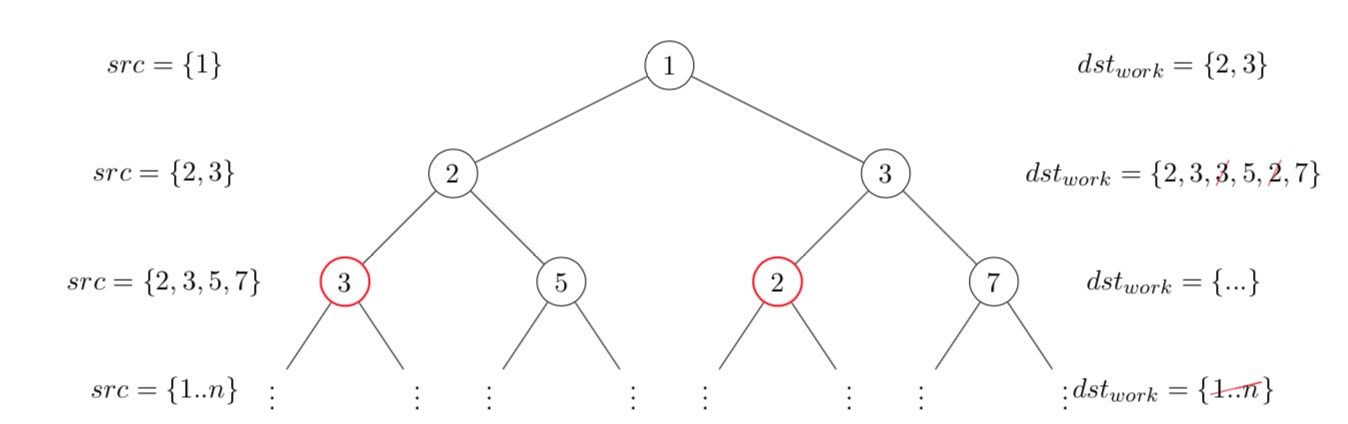
\includegraphics[width = \linewidth]{images/RecursiveSelect.jpg};
    \caption{Traversierung Standard SQL}
\end{figure}
Es wurde sich dafür entschieden den UNION Operator zu verwenden, um Duplikate innerhalb der Working Tabelle auszuschließen. Für die  Ergebnismenge der Abfrage auf der
relation Tabelle bedeutet dies, dass die Ergebnismenge ungefähr die Anzahl an Profilen haben sollte. Wohingegen die Abfrage mit UNION ALL, das Duplikate aus der
Working Tabelle nicht entfernt (\cite{postgresWithRecursive}), eine Ergebnismenge zurückliefert, die genauso viele Elemente hat wie die jeweilige relation Tabelle.

\subsection{Graphtraversierung mit Hilfe von verschachteltem SELECT Statement}
Bei der Graphtraversierung mit Hilfe von verschachteltem \ac{SQL} wird ein selbsterstelltes verschachteltest SELECT Statement verwendet. Ein Beispielstatement
befindet sich im Anhang (siehe \ref{SELECT}). Auf der obersten Rekursionsstufe wird der Startknoten des Graphen mitgegeben (in diesem Beispiel ist der Startknoten = 1).
Das Ergebnis dieser Abfrage wird als Eingabe für die nächst tiefere Rekursionstufe verwendet. In der WHERE Klausel wird für die Spalte src der IN Operator verwendet.
Der IN Operator erlaubt es, mehrere Werte innerhalb der WHERE Klausel anzugeben. Das DISTINCT in der SELECT Klausel sorgt dafür, dass Duplikate in der Ergebnissmenge
der momentanen Rekursionnstufe entfernt werden. Die Funktionsweise von DISTINCT ist in der folgenden
Grafik nochmal dargestellt:
\begin{figure}[H]
    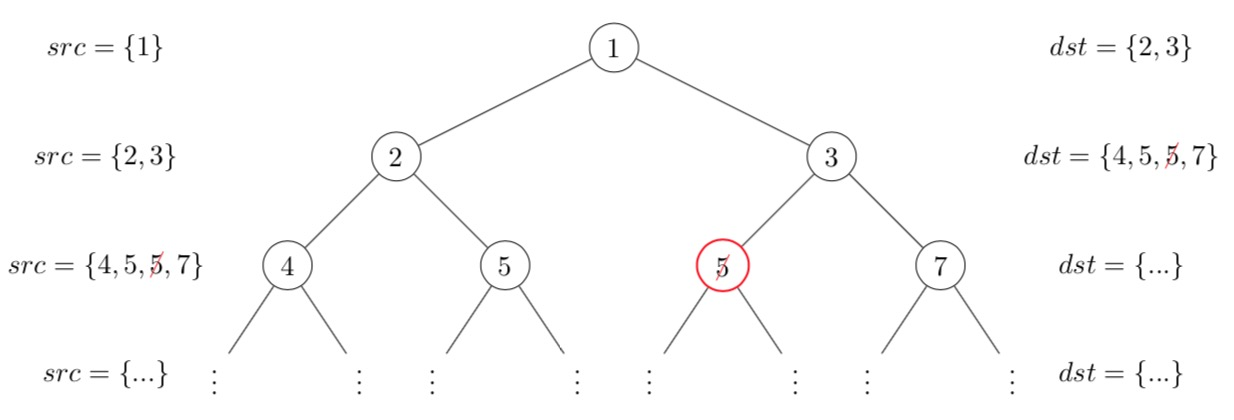
\includegraphics[width = \linewidth]{images/Distinct.jpg};
    \caption{Löschen von Duplikaten in einer Rekursionsstufe}
\end{figure}
Hierbei liegt der Knoten 5 so, dass er in der 2. Rekursionsstufe 2 Mal in der Auswahl auftaucht. DISTINCT entfernt das Duplikat. Die Ergebnismenge, entfernt um die
Duplikate, wird als Input für die nächste Rekursionsstufe verwendet.
Die Ausgabe des verschachtelten SELECT Statement sind die Nachbarn der Knoten, der angegebenen Rekursionstiefe. Wird zum Beispiel ein
verschachteltes SELECT Statement der Tiefe 3 erstellt, so gibt dieses Statement alle Nachbarn 3. Grades ausgehend vom Startknoten an. Der Nachteil bei dieser Methode ist, dass
Kreise in einem Graph nicht erkannt werden. Die Duplikatüberprüfung erfolgt nicht über mehrere Rekursionsstufen hinweg, sondern immer nur zwischen zwei Rekursionsstufen.

\subsection{Graphtraversierung mit Hilfe von rekursiven INNER JOIN}
Bei der Graphtraversierung mit Hilfe von rekursiven INNER JOIN soll der Graph traversiert werden, indem die Relationentabelle immer wieder mit sich selber verknüpft wird.
Die Ausgabe ist, ähnlich wie bei der Graphtraversierung mit Hilfe von verschachteltem SELECT Statement, die Nachbarn der Knoten, die sich auf der mitgegebenen Rekursionsstiefe
befinden. Ein Beispielstatement für den rekursiven INNER JOIN ist im Anhang gegeben (siehe \ref{JOIN}).

\subsection{Graphtraversierung mit Hilfe von selbstgeschriebenen Stored Procedure}
Bei der Graphtraversierung mit Hilfe von selbstgeschriebenen Stored Procedure wird der Graph mit Hilfe eines selbst erstellten Stored Procedure, das sich selber bis
zu einer mit gegebenen Rekursionstiefe wieder aufruft, traversiert (siehe \ref{recursiveFunction}). Die Abbruchbedingung wird dem Stored Procedure in Form einer
Rekursionsstiefe mitgegeben. In jeder Rekursionsstufe erstellt das Script 2 temporäre Tabelle. Eine temporäre Tabelle \footnote{Zuerst wurde das Script mit Hilfe einer standard Tabelle
erstellt. Dadurch war das Stored Procedure jedoch um den Faktor 7 langsamer. Es ist die Vermutung, dass durch die Anlage als temporäre Tabelle, die Tabelle im Shared Memory angelegt wird.
Hierdurch wird der Performancegewinn erzielt ( \cite[S.26]{froehlich01})}
wird auf Basis eines Eingabeparameter (Datenstruktur Array) erstellt.
Diese temporäre Tabelle besitzt eine Spalte. Diese Tabelle stellt die Spalte src der aktuellen Rekursionsstufe dar. Sie wird im IN Operator der WHERE Klausel verwendet
um die 2. temporäre Tabelle zu erstellen. Die 2. temporäre Tabelle beinhaltet die Spalte dst der aktuellen Rekursionsstufe. Die 2. temporäre Tabelle wird als
Aufrufparameter für die nächst tiefere Rekursionsstufe mitgegeben. In der nächst tieferen Rekursionsstufe dient die 2. temporäre Tabelle als die Tabelle, die alle
src Spalten der aktuellen Rekursionsstufe beinhaltet.
%\lstsetsql

%\end{figure}
%\subsection{Beurteilung}